\documentclass{ctexart}%ctexart中文编译

%%导言区，用于插入宏包
\usepackage{graphicx} % Required for inserting images
\usepackage{geometry} % 用于设置页边距
\usepackage{lastpage}
\usepackage{lipsum} %生成随机虚拟文本
\usepackage{fancyhdr} % 自定义页眉页脚
\usepackage{booktabs}%插入三线表
\usepackage{amsmath,amsfonts,amsthm}%数学常用
\usepackage{bm}%数学常用
\usepackage{mathrsfs}%数学用
\usepackage{listings}
\usepackage{xcolor}
\usepackage{ctex}


%%设置文章格式
\geometry{left=2.5cm,right=2.5cm,top=2cm,bottom=2cm}
\pagestyle{fancy}%输入empty就是不需要
\fancyhf{}
\lhead{}
\rhead{by air}
\cfoot{\protect 第\thepage 页}


%设置代码高亮格式
\definecolor{codegreen}{rgb}{0,0.6,0}
\definecolor{codegray}{rgb}{0.5,0.5,0.5}
\definecolor{codeblue}{rgb}{0,0,0.5}

\lstset{
  backgroundcolor=\color{white},   % 背景颜色
  commentstyle=\color{codegreen},  % 注释颜色
  keywordstyle=\color{codeblue},   % 关键词颜色
  stringstyle=\color{codegray},    % 字符串颜色
  basicstyle=\ttfamily\small,      % 字体和大小
  breaklines=true,                  % 自动换行
  numbers=left,                     % 行号在左
  numberstyle=\tiny\color{codegray},% 行号样式
  frame=single,                     % 加边框
  captionpos=b,                     % 标题在代码块底部
  tabsize=2,                        % 制表符大小
  language=C                        % 默认语言为C
}



\title{第二周：运算符}
\author{Air}

\begin{document}

\maketitle

\newpage
首先运算符顺序如下：

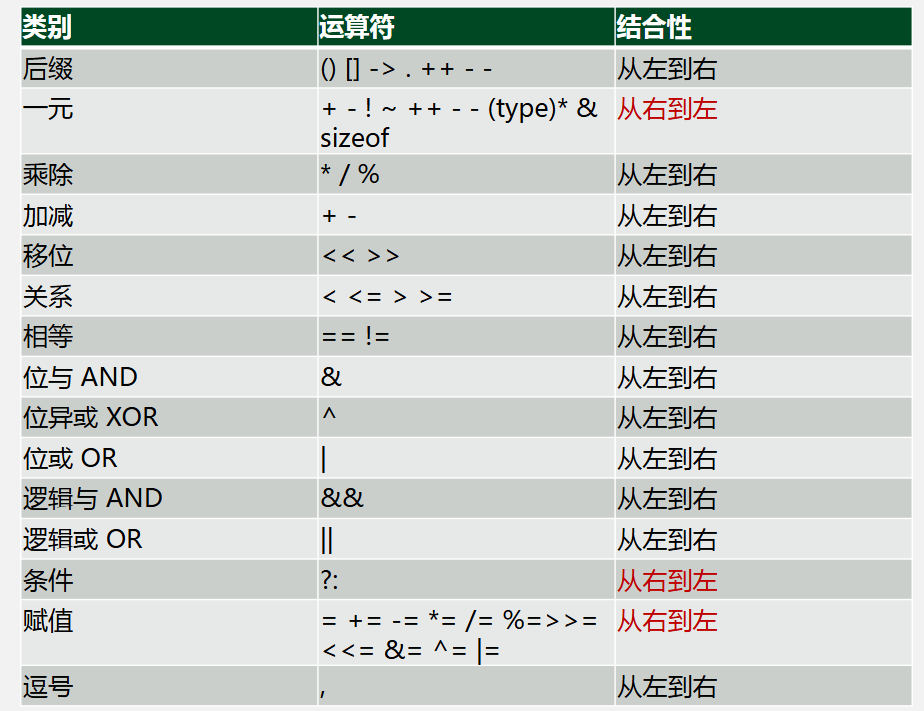
\includegraphics[width=0.8\textwidth]{image.png}


其次有个需要注意的是三元运算符，是就等于前者，否则等于后者

下面主要介绍一下位运算：

运用一：交换两个数
\begin{lstlisting}
#include<stdio.h>
int main(){
  int a,b,c;
  scanf("%d %d",&a,&b);
  a=a^b;
  b=a^b;
  a=a^b;

  printf("%d %d",a,b);
}
\end{lstlisting}

运用二：运算优化
\begin{lstlisting}
  #include<stdio.h>
  int main(){
    int a;int b;
    //a=257/8
    a=257>>8;
    //b=456%32;
    b=456-(456>>5<<5)；
  }
\end{lstlisting}

\newpage
运用三：定义掩码

\noindent 对于0000我们有：\begin{itemize}
  \item \&同化为0
  \item |不做处理
  \item \^不做处理
\end{itemize}
与此同时，对于1111：\begin{itemize}
  \item |同化为1
  \item \&不做处理
  \item \^用于求反
\end{itemize}
三个功能，同化，通过，求反。
\newpage

\end{document}